% Pollis drill-down: Help > Ask Pollis, questions about Pollis answered from its own documents, what it reads, how it
% finds the passages, how the answer is written and how models are compared (28 October 2026).
% For users who want the detail, and for whoever maintains Pollis.
% Written before the code, as Ask Pollis is to work: the specification to build it from. Check every statement against
% Pollis once it is built.
% Compile with: latexmk -pdf workflow_ask_pollis.tex
% Shared look for the one-page Pollis workflow handouts (same fonts and colours as the brochure).
\documentclass[10pt,a4paper]{article}

\usepackage[a4paper,left=17mm,right=17mm,top=14mm,bottom=16mm,footskip=8mm]{geometry}
\usepackage[T1]{fontenc}
\usepackage[default,semibold]{sourcesanspro}
\usepackage{microtype}
\usepackage{graphicx}
\usepackage[table]{xcolor}
\usepackage{tikz}
\usepackage[most]{tcolorbox}
\usepackage{fontawesome5}
\usepackage{enumitem}
\usepackage{fancyhdr}
\usepackage[hidelinks]{hyperref}

\graphicspath{{images/}}

% ---------------------------------------------------------------- colours (as in the brochure)
\definecolor{navy}{HTML}{1C3A5E}
\definecolor{pblue}{HTML}{3B78B5}
\definecolor{amber}{HTML}{F2B33D}
\definecolor{deepamber}{HTML}{D9902A}
\definecolor{pale}{HTML}{EEF3F9}
\definecolor{ink}{HTML}{2A2F36}
\definecolor{logonavy}{HTML}{173D63}
\definecolor{logodark}{HTML}{C98A1E}
\definecolor{logoamber}{HTML}{F2B446}
\definecolor{logocream}{HTML}{FEEFD2}
\definecolor{soft}{HTML}{5E6773}
\color{ink}

\setlength{\parindent}{0pt}
\setlength{\parskip}{3pt}
\setlist{nosep,leftmargin=*,itemsep=2pt}

\pagestyle{fancy}
\fancyhf{}
\renewcommand{\headrulewidth}{0pt}
\fancyfoot[L]{\footnotesize\color{soft}\textbf{Pollis}\enspace Bright Insights through Statistical Learning, Simulation and Optimisation}
\fancyfoot[R]{\footnotesize\color{soft}github.com/saragga/pollis/releases/latest}

% The Pollis logo, redrawn so it prints sharply at any size
\newcommand{\pollislogo}[1]{%
  \begin{tikzpicture}[x=#1/512,y=-#1/512,baseline=(current bounding box.center)]
    \fill[logonavy] (0,0) rectangle (512,512);
    \fill[logodark] (36,422) -- (104,256) -- (172,422) -- cycle;
    \fill[logoamber] (104,422) -- (203,180) -- (302,422) -- cycle;
    \fill[logocream] (203,422) -- (339,89) -- (476,422) -- cycle;
  \end{tikzpicture}}

% Top of the page: logo, name, kind of document (Workflow unless given, e.g. [Drill-Down]) and its subject;
% then the question and a one-line promise
\newcommand{\workflowhead}[4][Workflow]{%
  \thispagestyle{fancy}%
  \begin{minipage}[c]{13mm}\pollislogo{11mm}\end{minipage}%
  \begin{minipage}[c]{\dimexpr\linewidth-13mm\relax}
    {\color{navy}\Large\bfseries Pollis}\enspace{\color{soft}#1}\hfill
    {\color{deepamber}\small\bfseries\MakeUppercase{#2}}
  \end{minipage}\par\vspace{7mm}
  {\color{navy}\fontsize{22}{26}\selectfont\bfseries #3}\par\vspace{4pt}
  {\color{soft}\large #4}\par\vspace{5mm}}

% A menu path: \menu{Explore}{Access Data Libraries}... is written as \path{Explore \gt Access Data Libraries}
\newcommand{\gt}{\,{\color{deepamber}\bfseries ›}\,}
\newcommand{\menupath}[1]{{\footnotesize\bfseries\color{navy}#1}}

% A screenshot if images/<file> exists, otherwise an orange placeholder that says what to capture
\newlength{\shotheight}\setlength{\shotheight}{43mm}
\newcommand{\stepshot}[2]{%
  \IfFileExists{images/#1}{%
    \tcbox[enhanced, colback=black, colframe=black!70, boxrule=0.4pt, arc=2pt,
      left=0pt,right=0pt,top=0pt,bottom=0pt, boxsep=0pt, halign=center]{%
      \includegraphics[width=\dimexpr\linewidth-1pt\relax,height=\shotheight,keepaspectratio]{#1}}}{%
    \begin{tcolorbox}[enhanced, colback=white, colframe=orange!80, boxrule=0.6pt, arc=2pt,
      height=\shotheight, valign=center, halign=center, left=6pt, right=6pt]
      {\color{orange}\Large\faCamera}\par\smallskip
      {\color{orange}\footnotesize\bfseries Screenshot: #2}\par\smallskip
      {\color{orange!80!black}\scriptsize images/#1}
    \end{tcolorbox}}}

% One step: number, title, menu path, image file, what to capture, what it means
\newcommand{\step}[6]{%
  \begin{tcolorbox}
    {\color{deepamber}\Large\bfseries #1}\enspace{\color{navy}\large\bfseries #2}\par\vspace{1pt}
    \menupath{#3}\par\vspace{4pt}
    \stepshot{#4}{#5}\par\vspace{3pt}
    {\small #6}
  \end{tcolorbox}}

\newenvironment{steps}{%
  \begin{tcbraster}[raster columns=2, raster equal height=rows, raster column skip=4mm,
    raster row skip=4mm, enhanced, colback=pale, colframe=pale, boxrule=0pt, sharp corners,
    left=6pt,right=6pt,top=6pt,bottom=6pt, fontupper=\raggedright]}{\end{tcbraster}}

% Boxes for the bottom of the page
\newtcolorbox{pbox}[2][]{enhanced, colback=pale, colframe=amber, boxrule=0pt,
  leftrule=3pt, sharp corners, left=7pt, right=7pt, top=6pt, bottom=6pt,
  fontupper=\small\raggedright, before upper={{\color{navy}\normalsize\bfseries #2}\par\smallskip}, #1}
\newtcolorbox{nbox}[1][]{enhanced, colback=navy, colframe=navy, boxrule=0pt,
  sharp corners, left=8pt, right=8pt, top=6pt, bottom=6pt, coltext=white,
  fontupper=\small\raggedright, #1}

% A Next Steps item inside the bottom boxes
\newcommand{\nsitem}[2]{\item[\color{deepamber}\faChevronRight] \textbf{#1}: #2}


\usepackage{titlesec}
\usepackage{tabularx}
\usepackage{booktabs}
\usepackage{listings}
\usetikzlibrary{positioning,arrows.meta,fit}

\fancyhf{}
\fancyfoot[L]{\footnotesize\color{soft}\textbf{Pollis}\enspace Drill-down: Ask Pollis}
\fancyfoot[R]{\footnotesize\color{soft}\thepage}

\titleformat{\section}{\color{navy}\large\bfseries}{\color{deepamber}\thesection}{0.6em}{}
\titleformat{\subsection}{\color{navy}\normalsize\bfseries}{\color{deepamber}\thesubsection}{0.5em}{}
\titlespacing*{\section}{0pt}{12pt}{4pt}
\titlespacing*{\subsection}{0pt}{8pt}{2pt}
\setlength{\parskip}{4pt}

\lstset{basicstyle=\ttfamily\footnotesize, columns=fullflexible, keepspaces=true, breaklines=true,
  backgroundcolor=\color{pale}, frame=leftline, rulecolor=\color{amber}, framerule=2pt, xleftmargin=6pt,
  framexleftmargin=6pt, aboveskip=4pt, belowskip=4pt, upquote=true, tabsize=2}

\usepackage{xurl}
\newcommand{\file}[1]{{\small\nolinkurl{#1}}}
\newcolumntype{L}{>{\raggedright\arraybackslash}X}

\begin{document}

\workflowhead[Drill-Down]{Ask Pollis}
  {Questions about Pollis, answered from its own documents}
  {What Ask Pollis reads, how it cuts the documents into passages, how it finds the passages that answer a question,
   by their words and by their meaning, how the answer is written from them, on this computer or in the cloud, and
   where all of it is kept.}

\begin{nbox}
{\color{amber}\bfseries Drill-down.}\enspace
A look under the surface of \menupath{Help\gt Ask Pollis}. It is for anyone who wants to know why an answer says what
it says, and where it comes from, and for whoever maintains Pollis (\S\ref{sec:where} and \S\ref{sec:open} are for
them).
\end{nbox}

\tableofcontents

\section{Ask Pollis in one table}

Ask Pollis answers questions about Pollis: how to do something, where a menu item is, what a setting does, what a
panel computes. It answers only from Pollis's own documents, and every answer names the passages it rests on, so that
you can open them and check.

\begin{center}\small
\renewcommand{\arraystretch}{1.25}
\begin{tabularx}{\linewidth}{@{}p{0.27\linewidth}L@{}}
\toprule
Reads & The documents of \menupath{Help\gt Documentation}: the Tour, the Guide, A Tour of Pollis AI+, Pollis AI+,
  the drill-downs, the panel wikis, the package vignettes and the documents of the installed toolboxes\\
Finds passages by & their words (BM25, DuckDB's fts extension) and their meaning (embeddings, compared by cosine
  distance in DuckDB), the two lists merged\\
Answers with & a chat model on this computer, through the llama.cpp that comes with Pollis; or, if you choose, a
  cloud model with your own key\\
Keeps & one DuckDB file, \file{~/.pollis/ask/PollisAsk.duckdb}, a few megabytes\\
Sends out & nothing with a local model; with a cloud model, the question, the conversation so far and the passages
  found, never your files\\
Compares & chat models of your choice, local and cloud, on the same questions and the same passages, scored by a
  judge model (\S\ref{sec:compare})\\
Needs Julia & to build the index, in the background, and to compare models; asking does not\\
\bottomrule
\end{tabularx}
\end{center}

\section{The whole flow at a glance}

\begin{center}
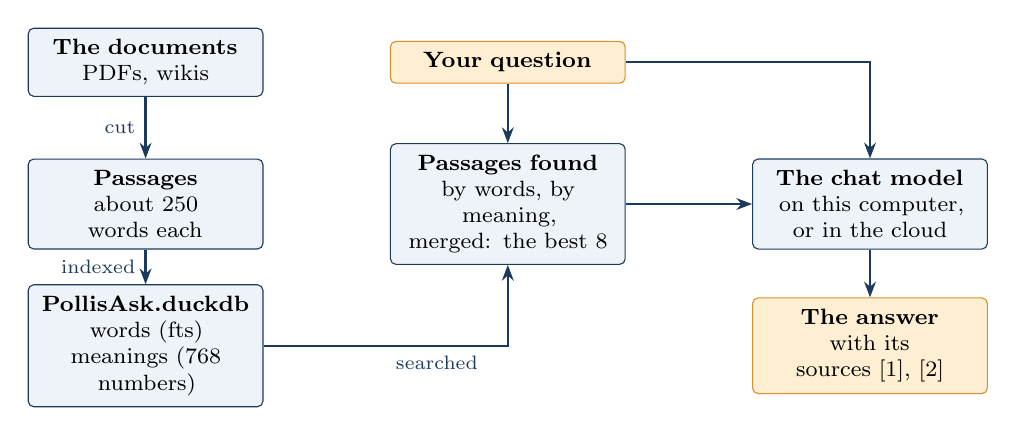
\begin{tikzpicture}[font=\footnotesize,
  box/.style={draw=navy, fill=pale, rounded corners=2pt, align=center, inner sep=4pt, text width=27mm},
  user/.style={box, draw=deepamber, fill=logocream},
  arr/.style={-{Stealth[length=2mm]}, navy, thick}]
  \node[box] (docs) at (0, 1.5) {\textbf{The documents}\\PDFs, wikis};
  \node[box] (passages) at (0, -0.3) {\textbf{Passages}\\about 250 words each};
  \node[box] (index) at (0, -2.1) {\textbf{PollisAsk.duckdb}\\words (fts)\\meanings (768 numbers)};
  \node[user] (question) at (4.6, 1.5) {\textbf{Your question}};
  \node[box] (found) at (4.6, -0.3) {\textbf{Passages found}\\by words, by meaning,\\merged: the best 8};
  \node[box] (model) at (9.2, -0.3) {\textbf{The chat model}\\on this computer,\\or in the cloud};
  \node[user] (answer) at (9.2, -2.1) {\textbf{The answer}\\with its sources [1], [2]};
  \draw[arr] (docs) -- node[left, font=\scriptsize] {cut} (passages);
  \draw[arr] (passages) -- node[left, font=\scriptsize] {indexed} (index);
  \draw[arr] (question) -- (found);
  \draw[arr] (index.east) -| node[below right, font=\scriptsize, pos=0.25] {searched} (found.south);
  \draw[arr] (found) -- (model);
  \draw[arr] (question.east) -| (model.north);
  \draw[arr] (model) -- (answer);
\end{tikzpicture}
\end{center}

The left column is built once, in the background, and again only for the documents that change. The right column runs
at each question, in a few seconds to some tens of seconds, depending on the model and the computer.

\section{Asking}\label{sec:asking}

\subsection{The page}
\menupath{Help\gt Ask Pollis} opens a page with a box for the question and \textbf{Ask}. The answer is written as it
comes, in a few paragraphs, with a number in brackets after each statement: \textbf{[1]}, \textbf{[2]}. Under it,
\textbf{Sources} lists the passages those numbers stand for, each with its document, its page or its wiki and heading,
and \textbf{Open}, which opens the document at that page or the panel's wiki at that heading.

\subsection{Following up}
Ask another question below the answer, and it is read with the conversation so far: \emph{and on Windows?} after a
question on installing a coding agent asks about installing it on Windows. \textbf{New Conversation} starts again with
nothing remembered. The conversation is kept only while the page is open.

\subsection{Answer With}
\textbf{Answer With}, beside the box, chooses the model that writes the answer:
\begin{itemize}
  \item \textbf{This Computer}, the default: the chat model of \file{pollis.ask.chatModel}, run by llama.cpp. Its name
    is shown, with the model picker of every local model input, and its first answer downloads it, once.
  \item \textbf{A cloud model}: Claude Haiku, Claude Sonnet, GPT-5.4 mini or GPT-5.5, with your own Anthropic or OpenAI
    key, kept in Pollis's secret storage. The key indicator beside the choice says whether a key is set.
\end{itemize}
The passages are always found on this computer, whichever model answers.

\begin{pbox}{What the questions are good for}
Ask Pollis knows what the documents say, and nothing else. It is good at \emph{how do I}, \emph{where is},
\emph{what does this setting do} and \emph{which panel computes}; it does not run code, look at your files or know
what Pollis did on your computer. When the documents do not answer a question, it says so, and lists the passages that
came closest.
\end{pbox}

\section{What it reads}\label{sec:reads}

\begin{center}\small
\renewcommand{\arraystretch}{1.25}
\begin{tabularx}{\linewidth}{@{}p{0.27\linewidth}LL@{}}
\toprule
\textbf{Document} & \textbf{Read from} & \textbf{Labelled with}\\
\midrule
The Tour, the Guide, A Tour of Pollis AI+, Pollis AI+ & their PDFs in \file{~/.pollis/documents}, compiled by Pollis &
  the document, the page, the topic of its spread\\
The drill-downs & their PDFs, the same way & the document, the page, the section\\
The panel wikis & the wiki files that come with Pollis, those written only & the panel, its menu, the wiki, the heading\\
The package vignettes & their PDFs, once compiled (opened once in Help\gt Documentation\gt Packages) & the package, the
  page, the section\\
The installed toolboxes & their documents and their panels' wikis & as above, with the toolbox's name\\
\bottomrule
\end{tabularx}
\end{center}

A wiki still \emph{Not written yet.} is left out: it would match questions about its panel with nothing to say. A
toolbox's passages come in when it is installed and go when it is removed.

\section{Cutting into passages}\label{sec:passages}

An answer can rest only on what reaches the model, and a whole document does not fit. So each document is cut into
\emph{passages}, small enough that a handful fit with the question, large enough that each says something whole.

\subsection{PDFs}
The text of each page is read with \file{pdftotext} (Poppler, through \file{Poppler\_jll}). A page's labels come from
the document's table of contents, which the compile keeps beside the PDF: the topic or section that is open on that
page. The page is then cut at its paragraphs into passages of up to about 250 words; a paragraph longer than that is
cut at a sentence. Each passage carries the last sentence of the one before it, so that a statement cut in two is
found whole in one of them. Page footers, the page numbers and the running titles are dropped.

\subsection{Wikis}
A wiki is Markdown: it is cut at its headings, and a section longer than about 250 words at its paragraphs, the same
way. A code block stays whole, and stays with the paragraph that introduces it. Tables are kept as rows of text, a
column's heading before each value, so that \emph{Default: 20} can be found under the right row.

\subsection{How many}
The documents of Pollis make between one and two thousand passages: the written panel wikis most of them, the Guide
about two hundred. The figure grows with the wikis written and the toolboxes installed.

\section{The index}\label{sec:index}

\subsection{One DuckDB file}
The passages are kept in \file{~/.pollis/ask/PollisAsk.duckdb}, on the DuckDB engine that comes with Pollis:

\begin{lstlisting}[language=SQL]
documents(id, kind, title, source, menu, toolbox, version)   -- one row per document read
passages(id, document, page, heading, text, embedding FLOAT[768])
built(name, value)          -- the embedding model, its prefixes, the Pollis version
\end{lstlisting}

\file{version} is the size and date of the file a document was read from, so that only the documents that changed are
read again (\S\ref{sec:fresh}).

\subsection{Words: the fts index}
DuckDB's full-text search extension, \emph{fts}, which comes with Pollis, indexes the heading and the text of each
passage:
\begin{lstlisting}[language=SQL]
PRAGMA create_fts_index('passages', 'id', 'heading', 'text', stemmer = 'english', overwrite = 1);
\end{lstlisting}
The English stemmer cuts words to their stems, so that \emph{filters} finds \emph{filter} and \emph{routing} finds
\emph{route}. Common words (\emph{the}, \emph{of}) are not indexed. The index takes a second or two to build.

\subsection{Meaning: the embeddings}
An \emph{embedding model} turns a text into a list of numbers, a point in a space where texts that mean the same are
close together, whatever their words. Each passage is given its point, 768 numbers, in the column \file{embedding}.
With EmbeddingGemma 2, the default (\S\ref{sec:models}), that space is the same for more than a hundred languages: a
question in Portuguese lands near the English passage that answers it.

The model is told what each text is, as it was trained to be. A passage is given to it as
\texttt{\small title: <its labels> \textbar{} text: <the passage>}, a question as \texttt{\small task: question answering \textbar{} query: <the question>}.
The two prefixes are settings (\S\ref{sec:settings}): another embedding model wants its own.

\subsection{How big}
Two thousand passages of 768 numbers take 6 MB, and comparing a question with every one of them takes milliseconds.
No vector index is needed: DuckDB reads them all, every time, and so never misses one. A vector index pays only beyond
about a million passages (\S\ref{sec:open}).

\section{Finding the passages}\label{sec:finding}

\subsection{Two searches}
Each question is searched twice:
\begin{itemize}
  \item \textbf{By words}: BM25, through the fts index, scores the passages that contain the question's words, the
    rarer a word in the documents, the more it counts. It is what finds an exact name:
    \file{pollis.agents.tierCells}, \emph{Snowball Search Map}, \emph{Install Skills}.
  \item \textbf{By meaning}: the question's embedding is compared with every passage's by cosine distance. It is what
    finds the passage that answers \emph{how do I make a cheap model do the small jobs?}, which has none of its words:
    it speaks of the Light tier of Model Tasks and Routing.
\end{itemize}
Each search keeps its best 20 passages.

\subsection{One list}
The two lists are merged by \emph{reciprocal rank fusion}: each passage scores $1/(60 + r)$ for its rank $r$ in each
list it is in, and the scores are added. A passage high in both comes first; a passage first in one list only still
does well. The ranks are used, not the scores, because a BM25 score and a cosine distance are not on the same scale. In
one query:

\begin{lstlisting}[language=SQL]
WITH words AS (
    SELECT id, row_number() OVER (ORDER BY score DESC) AS r
    FROM (SELECT id, fts_main_passages.match_bm25(id, $question) AS score FROM passages)
    WHERE score IS NOT NULL ORDER BY r LIMIT 20),
  meaning AS (
    SELECT id, row_number() OVER (ORDER BY array_cosine_distance(embedding, $vector::FLOAT[768])) AS r
    FROM passages ORDER BY r LIMIT 20)
SELECT id, sum(1.0 / (60 + r)) AS score
FROM (SELECT * FROM words UNION ALL SELECT * FROM meaning)
GROUP BY id ORDER BY score DESC LIMIT 8;
\end{lstlisting}

The best eight passages go to the model, about three thousand words in all. In a conversation, the question is searched
together with the one before it, so that \emph{and on Windows?} still finds the passages on installing an agent.

\section{Writing the answer}\label{sec:answer}

\subsection{What the model is given}
The model is given an instruction, the conversation so far, and the passages, each numbered and labelled:

\begin{lstlisting}
You answer questions about Pollis from the passages below, taken from its documentation.
Use only what the passages say. Name menus, buttons and settings exactly as the passages write them.
After each statement, cite the passages it rests on, as [1] or [1, 3].
If the passages do not answer the question, say so in one sentence, and name the passages that come closest.
Answer in the language of the question.

[1] The Pollis Guide, page 35, Orchestration > Model Tasks and Routing
Not every task needs the strongest model. Compose > Orchestration > Model Tasks and Routing has three tiers ...
\end{lstlisting}

\subsection{Why it can be trusted, and how far}
The answer can say only what the passages say, and each statement points to the passage it comes from: \textbf{Open}
shows it in its place. A small model can still join two passages wrongly, or miss the one that matters. When an answer
matters, open its sources. The documents themselves are checked against what Pollis does, release by release; an answer
is as current as the documents of the Pollis you run.

\subsection{Local or cloud}
On this computer, the model reads the passages and writes the answer without anything leaving it. A model with four
billion weights answers in a few seconds on Apple silicon or with a graphics chip, and in some tens of seconds on a
laptop without one, most of it spent reading the passages. A cloud model answers in a few seconds anywhere, and is
better at joining passages; it is sent the instruction, the conversation and the passages, which are Pollis's documents,
and your question.

\section{The models}\label{sec:models}

\begin{center}\small
\renewcommand{\arraystretch}{1.25}
\begin{tabularx}{\linewidth}{@{}p{0.18\linewidth}p{0.3\linewidth}lL@{}}
\toprule
& \textbf{Default} & \textbf{Download} & \textbf{Why}\\
\midrule
Embedding & EmbeddingGemma 2, Q8\_0 (Google) & 0.31 GB & 768 numbers per text; more than 100 languages; reads 8,192
  tokens; text, images, audio and video in one space\\
Chat & Qwen3.5 4B, Q4\_K\_M (Qwen) & 2.74 GB & follows long instructions, cites as asked, writes in many languages, on
  a laptop without a graphics chip\\
\bottomrule
\end{tabularx}
\end{center}

Both are GGUF files from Hugging Face, downloaded into \file{~/.pollis/models} the first time they are needed and listed
in \menupath{Compose\gt Local Models\gt Models Installed}. They are the defaults, not requirements: the model picker
offers every chat or embedding model on this computer, and \textbf{Add Model File...} any other. LLM Text Analysis
uses the same embedding model, so it is downloaded once for both.

Changing the embedding model computes every passage's embedding again, since the points of two models are not
comparable, and can change their length. Changing the chat model changes nothing in the index.

\section{Comparing models}\label{sec:compare}

Which model should answer: a small one that is quick, a larger one that is slower, or a cloud model? \textbf{Compare
Models...}, on the Ask Pollis page, answers that with figures, for the models you choose: any chat models on this
computer, of any size, and any cloud models with a key, such as Qwen3.5 0.8B, 4B and 9B against Claude Sonnet.

\subsection{Fair by construction}
Every model is given the same questions, the same passages and the same instruction (\S\ref{sec:answer}), so what is
compared is the model alone, and its answers are those Ask Pollis would give with it. The passages are found once per
question, on this computer, whichever models are compared. The local models run one after the other, each alone in
memory, so that none is slowed by another.

\subsection{One question, side by side}
\textbf{One Question} takes a question and shows each model's answer in a column of its own, with its sources and the
seconds it took. \textbf{Score These} then has the judge (\S\ref{sec:judge}) score each answer. It is the quick look:
how the answers differ, on a question that matters to you.

\subsection{A test set, scored}
\textbf{Test Set} runs many questions, and gives each model its figures. The questions come two ways:
\begin{itemize}
  \item \textbf{Made from the documents}: \textbf{Make Questions} takes 40 passages spread over the documents and has a
    model, Claude Sonnet by default, write for each a question that only that passage answers, and the answer. This is
    RAGTools.jl's \file{build\_qa\_evals}. It is done once, and kept.
  \item \textbf{Your own}: under an answer of Ask Pollis, \textbf{Add to the Test Set} keeps the question, with the
    answer you write and the source that holds it, chosen among its Sources.
\end{itemize}
\textbf{Run} then asks every question of every model chosen, and has each answer scored. A run of 40 questions on
three local models and a cloud one takes some minutes with a graphics chip or Apple silicon, and up to an hour on a
laptop without one. It runs in the background, with its progress shown, and \textbf{Stop} ends it with the questions
done kept.

\subsection{The figures}
\begin{center}\small
\renewcommand{\arraystretch}{1.25}
\begin{tabularx}{\linewidth}{@{}p{0.3\linewidth}L@{}}
\toprule
\textbf{Column} & \textbf{What it says}\\
\midrule
Model, Where, Size & the model, on this computer or in the cloud, and its download\\
Score & the mean of the judge's ratings, from 1 (worst) to 5 (best)\\
Relevance, Completeness, Clarity, Consistency, Helpfulness & the five parts of the rating, each from 1 to 5\\
Not Scored & the answers the judge could not rate, or the model did not give\\
Seconds & per answer, the mean, from the question sent to the last word\\
Tokens & per answer, read and written, for a cloud model what is paid for\\
\bottomrule
\end{tabularx}
\end{center}
Every run is kept, with its models, its judge and the Pollis it ran on, so that a run can be set beside an earlier one:
the same models after a new Pollis, or a new model against the old.

\subsection{The judge}\label{sec:judge}
The judge is a model that reads the question, the passages and an answer, and rates the answer: how relevant,
complete, clear and helpful it is, and how consistent with the passages, the five parts of RAGTools.jl's
\file{run\_qa\_evals}. It rates against the passages, not against the answer written with the question: an answer that
says what the passages say, in other words, scores as well. The judge is Claude Sonnet by default, and any chat model,
local or cloud, can be chosen; a small local model judges poorly. A judge may favour models of its own family, Claude
those of Claude, so a run can be scored by two judges, say Claude Sonnet and GPT-5.5, each in a column of its own.

\subsection{The passages found, and the embedding models}
For a question made from a passage, the run also checks whether that passage was among the eight found, and at what
place. That depends on the search, not on the chat model, so it is shown once, above the table: \emph{the right
passage among the eight for 34 of the 40 questions, at place 1.8 on average}. It is the figure that compares embedding
models: choose several, and each is given the passages once, in the comparisons' own file, and has its line.

\subsection{What a comparison sends out}
With local models only, and a local judge, nothing. With a cloud model or judge, what each is sent when it answers or
judges: the instruction, the question and the passages, which are Pollis's documents; and, to make questions, the 40
passages.

\section{Keeping the index up to date}\label{sec:fresh}

\subsection{When it is built}
The index is built by the hidden process of low priority that compiles the documents of Help\gt Documentation when the
Julia REPL starts, once they are compiled:
\begin{enumerate}
  \item The passages and the fts index, from the documents that are new or changed since the last time, in a few
    seconds. This needs no model, and nothing is downloaded.
  \item The embeddings of the new passages, the first time Ask Pollis is opened and every time after. The first time,
    this downloads the embedding model, 0.31 GB, and computes every embedding, a few minutes on a laptop without a
    graphics chip; then only the new passages', in seconds.
\end{enumerate}
The status bar shows \textbf{Indexing the documentation for Ask Pollis}, with the passages done.

\subsection{Before the embeddings are ready}
A question asked while the embeddings are being computed is searched by its words only, and the answer says so above
it. Most questions about a named menu item are answered as well; a question in other words, or in another language,
less well.

\subsection{What changes it}
A new Pollis, a wiki written, a vignette compiled, a toolbox installed or removed, or another embedding model. Nothing
else: your questions are not kept in the index, nor anywhere after the page is closed.

\section{When something goes wrong}

\begin{center}\small
\renewcommand{\arraystretch}{1.25}
\begin{tabularx}{\linewidth}{@{}p{0.4\linewidth}L@{}}
\toprule
\textbf{You see} & \textbf{What to do}\\
\midrule
\emph{The documentation is not indexed yet} & Start the Julia REPL, which compiles and indexes it; the status bar
  shows how far it has come.\\
\emph{Searched by words only: the embeddings are being computed} & Nothing: ask again in a few minutes for a search by
  meaning too.\\
\emph{The model could not be started} & Open \menupath{Compose\gt Local Models\gt Models Installed}, check that the
  model is there and that it fits in memory, or choose a smaller one, or a cloud model.\\
\emph{No key for Anthropic} (or OpenAI) & Set the key with the key indicator beside \textbf{Answer With}.\\
An answer that cites nothing & The passages did not answer the question; try the words the documents use, such as the
  name of the menu item.\\
\bottomrule
\end{tabularx}
\end{center}

\section{Settings}\label{sec:settings}

\begin{center}\small
\renewcommand{\arraystretch}{1.25}
\begin{tabularx}{\linewidth}{@{}p{0.36\linewidth}L@{}}
\toprule
\textbf{Setting} & \textbf{What it holds}\\
\midrule
\file{pollis.ask.answerWith} & This Computer, or the cloud model chosen in \textbf{Answer With}\\
\file{pollis.ask.chatModel} & The local chat model: \file{hf:unsloth/Qwen3.5-4B-GGUF/Qwen3.5-4B-Q4_K_M.gguf}\\
\file{pollis.ask.embeddingModel} & The embedding model: \file{hf:ggml-org/embeddinggemma-2-GGUF/embeddinggemma-2-Q8_0.gguf}\\
\file{pollis.ask.queryPrefix} & What a question is given to the embedding model as: \texttt{\small task: question answering \textbar{} query: \{text\}}\\
\file{pollis.ask.passagePrefix} & What a passage is given to it as: \texttt{\small title: \{title\} \textbar{} text: \{text\}}\\
\file{pollis.ask.passages} & How many passages go to the model: 8\\
\file{pollis.ask.compare.judges} & The judges of Compare Models: Claude Sonnet\\
\file{pollis.ask.compare.questionsBy} & The model that makes the questions of a test set: Claude Sonnet\\
\bottomrule
\end{tabularx}
\end{center}

\section{Where things are}\label{sec:where}

\begin{center}\small
\renewcommand{\arraystretch}{1.2}
\begin{tabularx}{\linewidth}{@{}p{0.47\linewidth}L@{}}
\toprule
\textbf{File} & \textbf{Role}\\
\midrule
\file{.../compose/browser/compose.contribution.ts} & Help\gt Ask Pollis\\
\file{.../compose/browser/askPollisPage.ts} & The page: the question, Answer With, the answer as it comes, Sources\\
\file{.../compose/node/askPollisMain.ts} & The DuckDB process that searches \file{PollisAsk.duckdb} (\S\ref{sec:finding})\\
\file{extensions/language-julia/src/pollisDocuments.ts} & Starts the indexing after the documents are compiled\\
\file{.../terminalserver/ask\_index.jl} & Reads, cuts and indexes the documents, and computes the embeddings\\
\file{extensions/language-julia/src/pollisLlamaServer.ts} & Runs the embedding and the chat model with llama-server\\
\file{.../compose/browser/media/askPollisPrompt.md} & The instruction of \S\ref{sec:answer}, the same for Ask Pollis
  and Compare Models\\
\file{.../compose/browser/compareModelsPage.ts} & Compare Models: One Question, Test Set, the runs\\
\file{extensions/language-julia/src/pollisCompareModels.ts} & Runs a comparison in a Julia process of its own, each
  local model in turn\\
\file{.../terminalserver/ask\_compare.jl} & Makes the questions, asks them, and has them judged, with RAGTools.jl\\
\file{~/.pollis/ask/PollisAsk.duckdb} & The index\\
\file{~/.pollis/ask/Comparisons.duckdb} & The test sets, the runs, their answers and scores, and the passages'
  embeddings of the embedding models compared\\
\bottomrule
\end{tabularx}
\end{center}

\section{Open points}\label{sec:open}
\begin{itemize}
  \item \textbf{Your own library}: your articles and books, as PDFs, and the works of PollisReferences, are the next
    corpus. They would be a second index beside Pollis's, with a choice of what to ask.
  \item \textbf{Voice, images and video}: EmbeddingGemma 2 already places images, audio and video in the same space as
    text, so they can join the index without another model. Beyond about a million passages, comparing every one
    becomes slow, and a vector index pays: DuckDB's VSS extension, whose index on disk is still experimental, or the
    Lance format.
  \item \textbf{RAGTools.jl and PromptingTools.jl in Compare Models only}: asking does not use them. DuckDB does the
    storing and both searches, and llama-server the models, so a framework would add little; the answer is asked for
    by Pollis itself, and the index needs only llama-server's embeddings, one request each. Compare Models uses
    RAGTools.jl for its \emph{evaluation}, a set of test questions whose right passages and answers are known, to
    measure whether the right passages are found and the answers keep to them, and so to compare models and settings
    by their scores (\S\ref{sec:compare}); and PromptingTools.jl, which RAGTools.jl calls the models with. Both are
    Pollis's forks, which run on Julia 1.13, as in LLM Text Analysis. RAGTools.jl also has a \emph{reranker}, a second
    model that reads the question with each of the best twenty passages and chooses the eight again, better, at the
    cost of some seconds. RAGTools.jl could come into Ask Pollis later, for reranking.
  \item \textbf{Test sets in English}: the questions made from the documents are in English, as the documents are; a
    test set in another language would show how well each model answers in it.
  \item \textbf{One stemmer}: the search by words stems English only; a question in another language is found by its
    meaning.
  \item \textbf{No reranker}: the eight passages are those of the merged ranks. A model that reads the question with
    each passage and scores it again would choose better, at the cost of a second model and some seconds.
  \item \textbf{Vignettes not opened}: a package vignette is read only once it has been compiled.
\end{itemize}

\end{document}
